\chapter{Introduction}
\label{chap:introduction}

\section{Context}

Quality control plays an important role in large-scale software development. The number of coding errors are noticeably increasing with the number of contributors. The more developers work together on developing a software, the more versatile their coding styles and conventions are.

To ensure the quality of the source code, thus the software itself, and at the same time help developers with their tasks, the need arises for a solution continuously reviewing the code, searching for mistakes, and enforcing conventions.

% \begin{figure}[!ht]
% 	\centering
% 	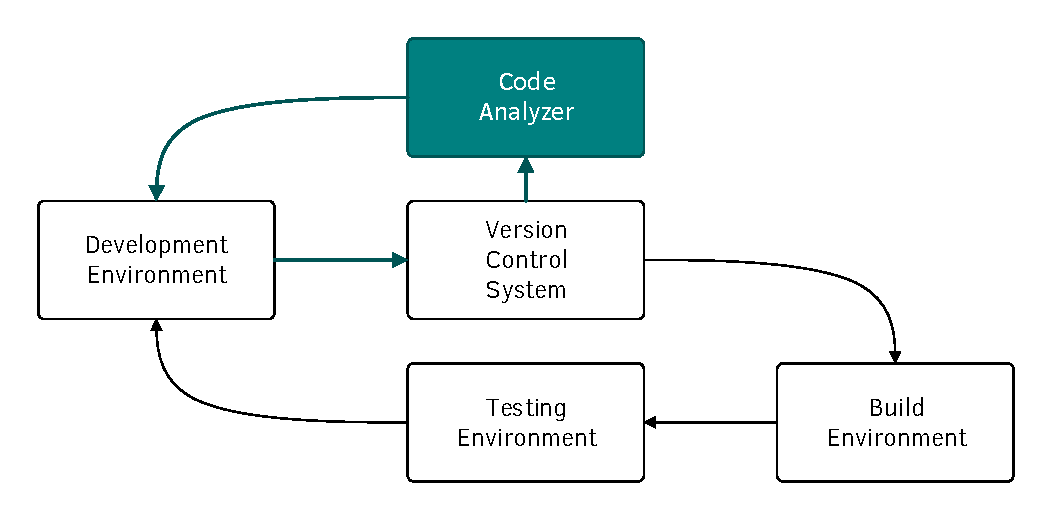
\includegraphics[height=6cm]{CI-workflow}
% 	\caption{Continuous Integration workflow extended with Static Analysis.}
% 	\label{fig:CI-workflow}
% \end{figure}


Version control systems (VCS) and continuous integration (CI)~\cite{CI} are widely used tools of the modern software developers. \Cref{fig:CI-workflow} shows an extended version of the generally used continuous integration workflow.
The basic workflow consists of the following steps. The developer makes modifications to the codebase using their \textit{Development Environment}. The modifications are committed into a \textit{Version Control System}, and this commit triggers the \textit{Build Environment} to build the project. The \textit{Testing Environment} can then perform runtime tests on latest build of the project. After this process, the results --- build and test logs --- are presented to the developer.

These logs help the developers discover bugs and failures before the software is released for manual testing or production purposes. Producing this information and making sure the software is working as intended often and early in the development workflow is vital for agile development.

A proven method of enhancing software quality is utilizing static program analysis techniques supplementing the basic CI workflow. During this method, the code is analyzed without executing the application. In practice, this method is able to reveal problems that are undetectable with testing and thus is able to aid the developer in creating higher quality software.


\section{Problem Statement}

Static analysis methods verifying that the code is compliant with coding conventions are often time consuming and resource intensive in practice. The size of the codebase may require a scalable solution, especially for continuous integration purposes, since the entire verification process needs to be carried out on the whole codebase once it is (partially) modified.

A temporary solution to tackle this problem is to process the changes in batches. To save resources, static analysis runs are carried out for a joined group of changes, rather than for every individual commit.

In an ideal situation, even before committing the changes, the developers receive feedback about the problems their modifications would imply.


\section{Objectives and Contributions}

My main objective is to provide a solution for reducing the time required for global, codebase-level reevaluation of static analysis after a change occurs.

I aim to create a framework, that transforms the whole source code repository into a graph representation and maintains it afterwards. It can perform code convention compliance checks, execute built-in static analysis tests and be extended with arbitrary tests by the user.




Incremental processing is one of the possible solutions for speeding up static analysis. In this thesis I present a system that is able to search for coding problems based on high level specifications expressed with graph patterns. By processing source repository changes and mapping them efficiently to stages of the processing workflow, the system supports incremental evaluation. Hence, after the initial query evaluation and report generation, consecutive runs are significantly more efficient.


Also, it should be able to process a subset of the repository, e.g. only the modifications introduced by the latest commit. This way, the system will be capable of incrementally processing the modifications in a commit. In this context, incremental processing means that only the modifications and their effects are merged into a continuously stored and updated report of the source project.

This framework requires a backend, e.g. a version control system, that is capable of sending notifications of the changes in the source code repository. Version control systems are not only able to provide the latest or the earlier revisions of the code, but also the changes that happened between revisions.

Our framework uses a dedicated component to determine the effects of the changes in addition to the changes provided by the version control system. This component also calculates the source code artifacts that have to be reprocessed with static analysis. This way, we only have to work on a subset of the source code, instead of reprocessing the whole project after a modification occurs.

In order to evaluate our framework, we created a benchmarking environment and conducted measurements on open-source software repositories.



\section{Structure of the Thesis}
